% begin module area-between-curves-ex1
\begin{frame}
\begin{example}%[Example 1, p. 348]
Find the area of the region bounded above by $\alert<handout:0| 3>{y = x^2 + 1}$, bounded below by $\alert<handout:0| 4>{y = x}$, and bounded on its sides by $\alert<handout:0| 6>{x = 0}$ and $\alert<handout:0| 6>{x = 1}$.
\begin{columns}
\column{.4\textwidth}
\ \only<handout:0| -2>{%
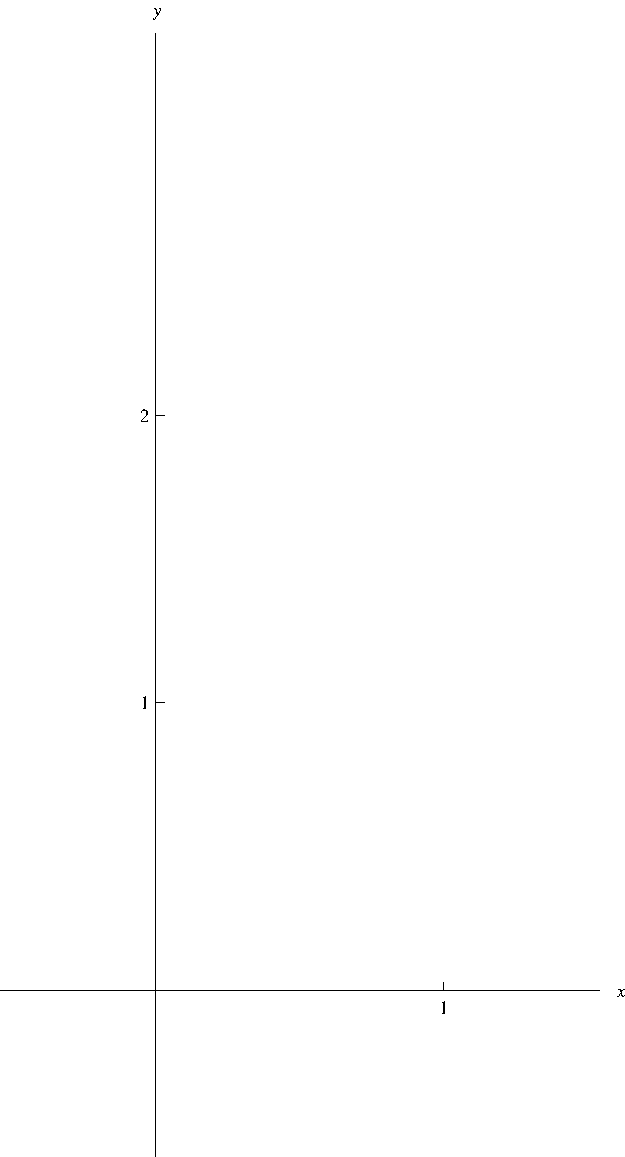
\includegraphics[height=6.5cm]{area-between-curves/pictures/06-01-ex1a.pdf}%
}%  
\only<handout:0| 3>{%
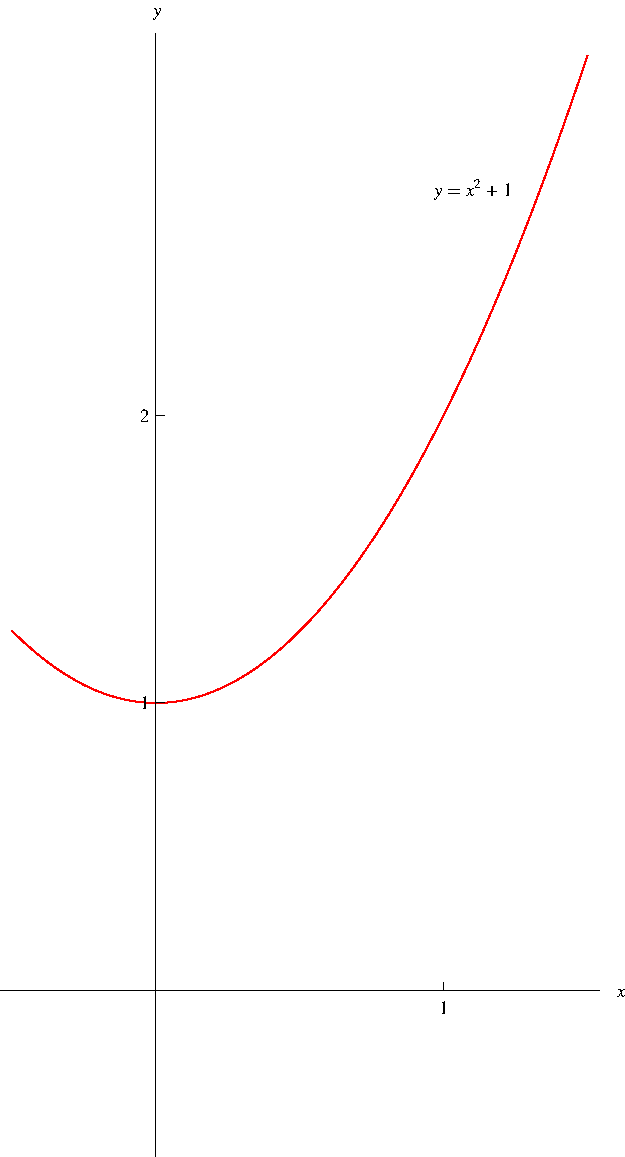
\includegraphics[height=6.5cm]{area-between-curves/pictures/06-01-ex1b.pdf}%
}%  
\only<handout:0| 4-5>{%
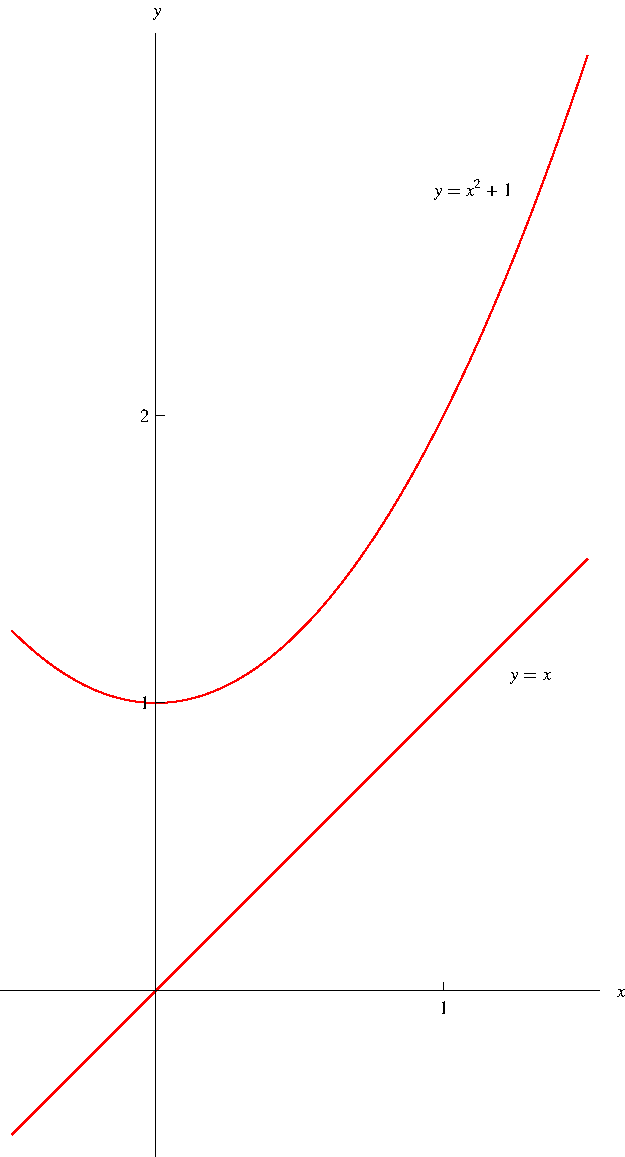
\includegraphics[height=6.5cm]{area-between-curves/pictures/06-01-ex1c.pdf}%
}%  
\only<6->{%
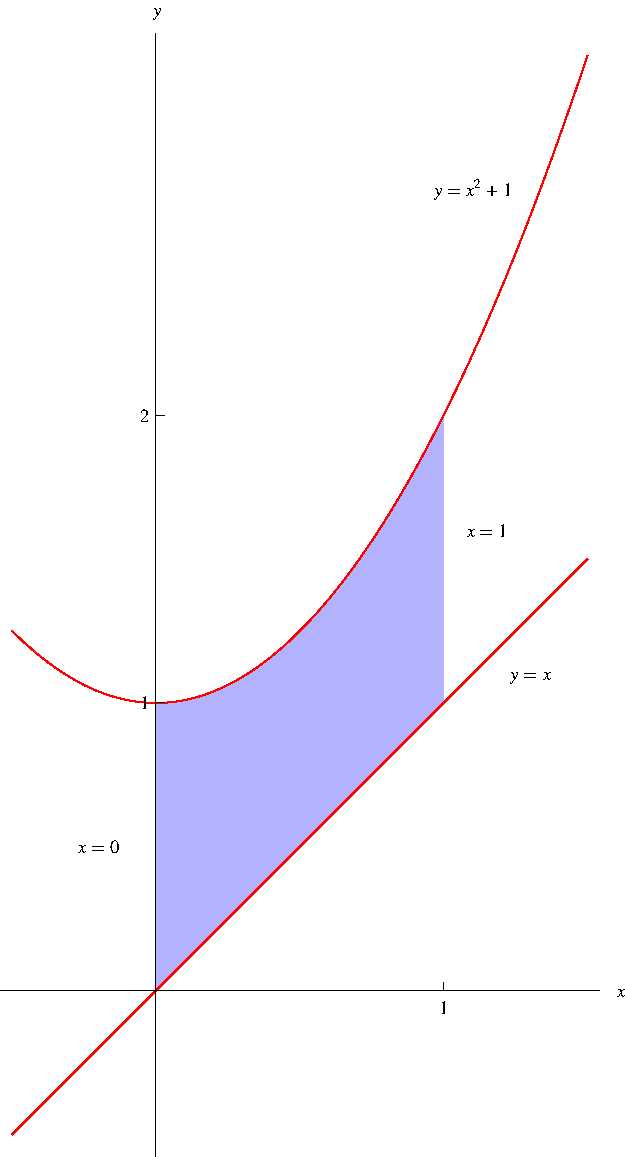
\includegraphics[height=6.5cm]{area-between-curves/pictures/06-01-ex1d.pdf}%
}%  

\column{.6\textwidth}
\begin{enumerate}
\item<2->  Graph the functions.
\item<5->  Identify the region.
\item<7->  Integrate.
\end{enumerate}
\abovedisplayskip=0pt
\belowdisplayskip=0pt
\abovedisplayshortskip=0pt
\belowdisplayshortskip=0pt
\begin{align*}
\uncover<8->{A} & \uncover<8->{=}  \uncover<8->{\int_0^1 |(x^2 + 1) - x|\diff x} \\
 &  \uncover<8->{=}  \uncover<8->{\int_0^1 ( x^2 - x + 1 ) \diff x} \\
 & \uncover<9->{=}  \uncover<9->{\left[  \frac{x^3}{3} - \frac{x^2}{2} + x \right]_0^1} \\
 & \uncover<10->{=}  \uncover<10->{ \frac{1}{3} - \frac{1}{2} + 1 } \uncover<11->{  = \frac{5}{6}. } 
\end{align*}
\end{columns}
\end{example}
\end{frame}
% end module area-between-curves-ex1
